\subsection{Setup Pengujian}
\label{subsection:setup-pengujian}

Sistem yang digunakan dalam pengujian dan juga \textit{benchmark} memiliki konfigurasi yang ditentukan pada file konfigurasi ./etc/config.json. Konfigurasi ini sebelumnya sudah dijelaskan sebagian pada bagian \ref{subsubsection:implementasi-benchmark}.

Untuk masing-masing node, konfigurasi yang ada adalah \textit{ip}, \textit{port}, \textit{port http}, \textit{path} untuk \textit{transaction log}, dan \textit{path} untuk data persisten \textit{key-value store database}. Konfigurasi global yang ada selain konfigurasi masing-masing node adalah \textit{storage}, yaitu jumlah \textit{data shard} dan \textit{parity shard} untuk erasure coding serta ukuran \textit{payload} maksimal yang akan diterima sistem. File konfigurasi yang digunakan dapat dilihat pada gambar \ref{fig:config-json}.

\begin{figure}[ht]
    \centering
    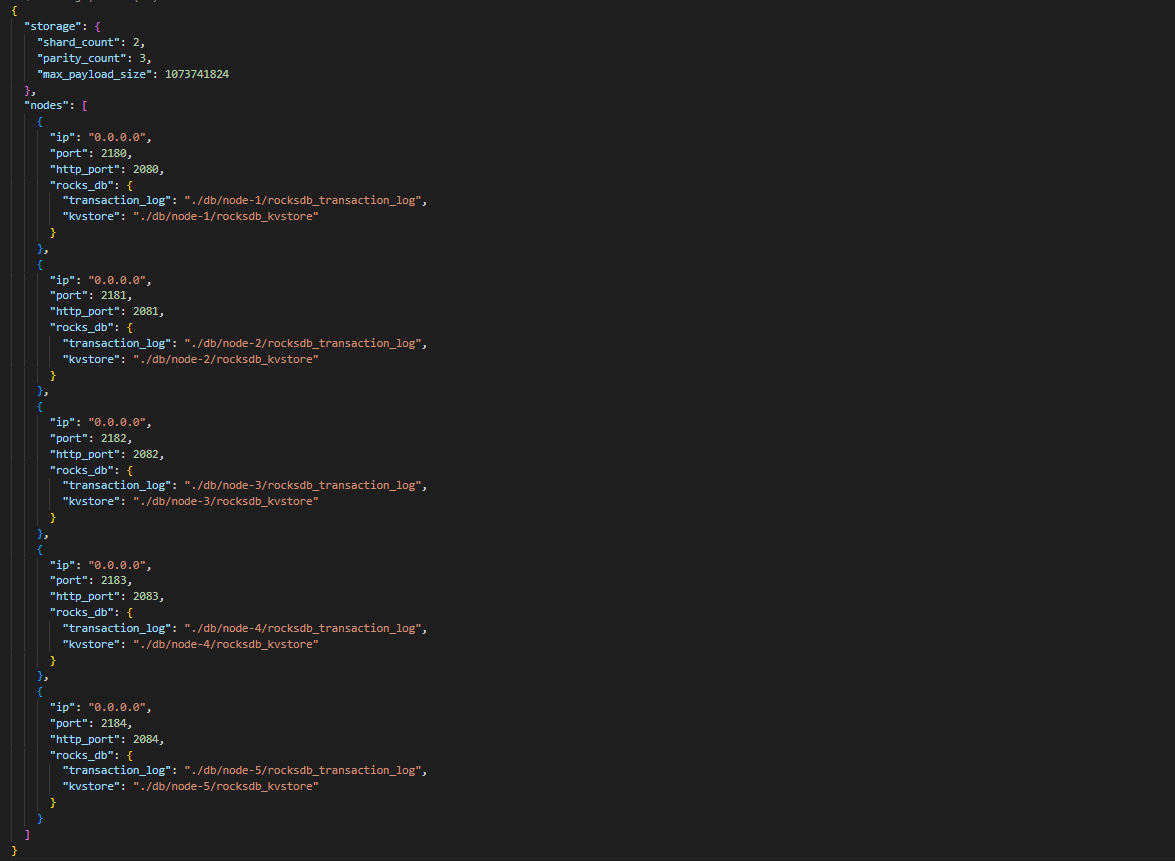
\includegraphics[width=0.95\textwidth]{resources/chapter-4/konfigurasi.png}
    \caption{File konfigurasi yang digunakan}
    \label{fig:config-json}
\end{figure}

Pengaturan sistem untuk menggunakan \textit{erasure coding} atau replikasi tidak ditentukan pada file konfigurasi, tetapi dilakukan saat menjalankan sistem. Pengguna dapat memilih untuk menggunakan \textit{erasure coding} atau
replikasi dengan menggunakan \textit{flag}. Dengan demikian, konfigurasi yang digunakan untuk \textit{erasure coding} dan replikasi adalah sama. Untuk replikasi, jumlah \textit{data shard} dan \textit{parity shard} akan diabaikan dan jumlah keduanya akan dianggap sebagai jumlah \textit{node} secara keseluruhan.

Setup dari sistem dilakukan dengan menjalankan perintah pada file scripts.sh yang sudah disebutkan pada bagian \ref{subsubsection:implementasi-benchmark}, yaitu run\_all. Perintah ini akan menjalankan semua \textit{node} dari sistem \textit{key-value store database} sesuai dengan konfigurasi yang telah ditentukan pada file ./etc/config.json dengan fitur \textit{erasure coding} diaktifkan dengan menambahkan \textit{flag} --erasure. Selain itu, \textit{flag} --trace dapat digunakan untuk mengaktifkan \textit{tracing} pada sistem. Pengaktifan \textit{tracing} akan menghasilkan log yang dapat digunakan untuk analisis lebih lanjut.